%\documentclass[sigconf]{acmart}
\documentclass[sigconf,anonymous,10pt]{acmart}
\usepackage{graphicx}
\graphicspath{ {./images/} }

% Copyright
% Pick the correct copyright notice that matches your rights form
%\setcopyright{none}
\setcopyright{acmcopyright}
%\setcopyright{acmlicensed}
%\setcopyright{rightsretained}
%\setcopyright{usgov}
%\setcopyright{usgovmixed}
%\setcopyright{cagov}
%\setcopyright{cagovmixed}

% DOI
%\acmDOI{10.475/1234.5678}

% ISBN
%\acmISBN{123-4567-24-567/08/06}

%Conference
\acmConference[SYSTOR'21]{ACM International Systems and Storage Conference}{June 14-16, 2021}{Haifa, Israel}
\acmYear{2021}
\copyrightyear{2021}

%\acmArticle{4}
\acmPrice{15.00}

% These commands are optional
%\acmBooktitle{Proccedings of the ACM International Systems and Storage Conference}
%\editor{John Doe}
%\editor{Jane Doe}

\begin{document}

\title{Position: CRDTs for truly concurrent file systems}

% Fill in your details. The \documentclass "anonymous" parameter keeps them hidden, remove it after the review process finishes
\author{Romain Vaillant}
\affiliation{%
  \institution{Scality}
  \city{Paris}
  \state{France}
}
\email{romain.vaillant@scality.com}


% The default list of authors is too long for headers.
\renewcommand{\shortauthors}{R. Vaillant et al.}

\begin{abstract}
Building scalable and highly available geo-replicated file systems is hard.
These systems need to resolve conflicts that emerge in concurrent operations in a way
that maintains the file system invariants, is meaningful to the user,
and does not depart from the traditional file system interface.
Conflict resolution in existing systems often leads to unexpected or inconsistent
results.
This paper presents the design of ElmerFS, a geo-replicated, truly concurrent
file system built with the aim of addressing these challenges.
Conflict resolution in ElmerFS is designed with the principle of preserving
user intention.
File system replicas converge to a common state through the use of Conflict-free
replicated data types (CRDTs) for representing file system structures.
The resulting state informs the user about the resolved conflict in an intuitive way.
The user can then complement or reverse the conflict resolution outcome using
traditional file system operations.
We demonstrate this mechanism through conflict resolution examples.
% the problem of building highly available shared and
% geo-replicated distributed POSIX file systems (FS).
% We explore the path of building a distributed file system that
% is geo-distributed, highly resilient and scalable by
% using Conflict-free Replicated Data Types (CRDTs) i.e. replicated data
% structures that do not need any coordination. We build upon these data
% structures and explore solutions to ensure that the application remains correct and in a final state that keeps the original user intention in case of conflicting operations.

\end{abstract}

%% Note: Classification and Keywords are only required for the camera-ready version

%
% The code below should be generated by the tool at
% http://dl.acm.org/ccs.cfm
% Please copy and paste the code instead of the example below.
%
\begin{CCSXML}
	<ccs2012>
	   <concept>
		   <concept_id>10010520.10010575.10010755</concept_id>
		   <concept_desc>Computer systems organization~Redundancy</concept_desc>
		   <concept_significance>500</concept_significance>
		   </concept>
	   <concept>
		   <concept_id>10011007.10011074.10011075.10011077</concept_id>
		   <concept_desc>Software and its engineering~Software design engineering</concept_desc>
		   <concept_significance>300</concept_significance>
		   </concept>
	   <concept>
		   <concept_id>10011007.10011074.10011075.10011077</concept_id>
		   <concept_desc>Software and its engineering~Software design engineering</concept_desc>
		   <concept_significance>300</concept_significance>
		   </concept>
	   <concept>
		   <concept_id>10010520.10010521.10010537.10010538</concept_id>
		   <concept_desc>Computer systems organization~Client-server architectures</concept_desc>
		   <concept_significance>300</concept_significance>
		   </concept>
	   <concept>
		   <concept_id>10010520.10010575.10010578</concept_id>
		   <concept_desc>Computer systems organization~Availability</concept_desc>
		   <concept_significance>500</concept_significance>
		   </concept>
	   <concept>
		   <concept_id>10010520.10010575.10010577</concept_id>
		   <concept_desc>Computer systems organization~Reliability</concept_desc>
		   <concept_significance>500</concept_significance>
		   </concept>
	 </ccs2012>
\end{CCSXML}

\ccsdesc[500]{Computer systems organization~Redundancy}
\ccsdesc[300]{Software and its engineering~Software design engineering}
\ccsdesc[300]{Software and its engineering~Software design engineering}
\ccsdesc[300]{Computer systems organization~Client-server architectures}
\ccsdesc[500]{Computer systems organization~Availability}
\ccsdesc[500]{Computer systems organization~Reliability}

% \keywords{ACM proceedings, \LaTeX, text tagging}

\maketitle

\sloppy

\section{Introduction}

File systems services are essential for data sharing and collaboration among users.
These services must provide low response time, remain available in the persistence
of network partitions, and provide support for offline work \cite{howard1988scale}.
To achieve these goals, these services typically rely on systems that replicate
data among geographically distant sites and serve each user request from the replica
closer to the user, without coordination with other replicas.

This type of design allows replicas to accept concurrent operations that conflict
with one another, for example concurrently creating two files with the same name
under the same directly on two different replicas.
As a result, these systems face two challenges:
resolving conflicts between concurrent operations in a way that is meaningful to
the users while maintaining file system invariants,
and ensuring support for legacy applications that have not been developed with
mechanisms for dealing with concurrency anomalies.

It has been shown that existing file system services that support collaboration
and offline work merge some conflicts in inconsistent, non-deterministic or
unexpected ways \cite{cai2018some, taothanh:tel-01673030}.
For example, in Google Drive the conflict described above can result in two
replicas presenting two different views of the file system to users.

This makes it difficult for users to have an intuitive understanding about
the behaviors of these services,
leading to misconceptions on their expected behavior~\cite{tang2013you}.
Moreover, enabling more flexible conflict resolution by exporting some decisions
to the users while maintaining support for legacy applications through POSIX
compliance is challenging.

In this paper, we present a comprehensive analysis of the challenges in the
design of geo-replicated weakly consistent file systems.
Guided by this analysis, we propose ElmerFS,
a geo-replicated file system that provides intuitive conflict resolution
semantics, while maintaining support for legacy applications.
The design of ElmerFS leverages the properties of Conflict-free replicated data
types (CRDTs) to ensure that concurrent operations on different replicas always
converge into a consistent state.
The guiding design principle is that conflict resolution should preserve user
intention.
Finally, we demonstrate through conflict resolution examples that a CRDT-based
file system design can provide conflict resolution semantics that are intuitive
to the user.

\section{Designing a file system}

\subsection{File system invariants}

POSIX's file systems organize files and directories in a tree structure.
To design our file system we focus on the following tree invariants:

\begin{enumerate}
\item Tree nodes are always reachable from the root directory.
\item Directories can have at most one parent node.
\item Cycles are possible only through symbolic links.
\end{enumerate}

We categorize two types of operations.
Structural operations, which can be used to manipulate the file system
structure (the tree), and content operations,
which can be used to store and retrieve information from files.

File systems are commonly represented internally as a collection of inodes.
We do not depart from this representation:
An inode represents a file system object (file, directory or symbolic link).
Each inode is identified by a unique numeric identifier (an ino).
A link is a reference to an inode. A directory entry is a named and visible representation of a link.

\subsection{File systems under weak consistency}
\label{fs:weak}

Preserving file system invariants in a replicated file system
that allows updates in multiple replicas with coordination
among them presents several challenges:

\begin{itemize}
	\item \textbf{Unique identifiers}: Any operation that creates
	inodes needs to generate a unique identifier.
	Without coordination among replicas, generated ids might conflict.
	In practice, this is addressed using 16 byte ids.
	However, this is not compatible with the POSIX specification, which requires 8 byte ids.
	\item \textbf{Named links}: Operations that create or move objects (files or directories)
	may result in conflicts in which concurrent operations οn different replicas create
	objects with the same name in the same directory.
	Existing systems resolve naming conflicts between files by automatically renaming
  files, and conflicts between directories either by renaming or by merging them.
	\item \textbf{Preserving the FS tree invariants}: Concurrent move
	operations without coordination may violate the file system invariant.
  For example, merging an operation that moves a directory A into a
	directory B with a concurrent operation that moves B into A can result in a cycle.
  Merging two concurrent operations that move the same directory
	to different destinations can result in a directory with two parents.
  \item \textbf{Deletion of inodes}: Concurrent link and unlink operations may result in different behavior depending on the order in which operations are applied on each replica.
  % The file system may be left with a partial inode that is not fully deleted but apparent.
  Moreover, even if a common conflict resolution is applied to all replicas, the
  result might not be what the user expects from the system.
  \item \textbf{Permissions changes}: Updating permission from a replica may not
  be propagated directly to other replicas.
  Merging an operation that removes a Bob's permission to write to file with a
  concurrent operation in which Bob writes
  to that file will result in a different outcome depending on the order in which
  operations are applied.
  % (This is very interesting but can create a lot of questions, it's maybe better to avoid mentioning permissions)
\end{itemize}

\subsection{Conflict-Free Replicated Data Types}

Ensuring that all replicas converge to the same state without coordination
is not trivial.

Conflict-Free Replicated Data Types (CRDTs) are data structures that
can be replicated across multiple replicas, and these replicas can be updated independently and concurrently without coordination.

By construction, CRDTs guarantee that modifications on different
replicas can always be merged into a consistent state without requiring
any special conflict resolution code or user intervention.

Moreover, the rules used for conflict resolution are parts of each CRDT's
definition.
Therefore, application developers can control their conflict resolution semantics by
choosing the types of CRTDs they model their application with.

\subsection{Assumptions and objectives}

We want to leverage CRDTs to develop a file system that is always available
and that provides good response times whatever the network conditions.
It must support active/active configurations
(i.e. two geographically distant clusters can issue read, write and structural
operation at the same time without coordination with each other).

Given the requirements, we want to keep the behavior of the file system as
close as possible to a local file system.
In summary, we want the following properties:

\begin{itemize}
	\item \textbf{Preserve intention}: We minimize changes not initiated by the user.
	The user should to be able to develop a simple mental model to understand
	the underlying convergence properties.
	\item \textbf{Truly concurrent operations}: One way to handle concurrency
	is to use consensus to serialize operations applied on the relevant objects.
	CRDTs avoid this and allow true concurrency without the need for
	a consensus.
	\item \textbf{Follow the POSIX standard}.
	\item \textbf{Atomic operation}: No matter how complex a FS operation is,
		  it should be either performed are completely discarded.
	\item \textbf{Always available}: CRDT types permit the design of design systems that
	are always available even under extreme network conditions.
	\item \textbf{Active-Active}: Several replicas accept operations
	(structural and updates) concurrently and propagate them from one-another,
	even after long delays.
\end{itemize}

A Focus has been placed on building on CRDTs to create a highly resilient and truly
concurrent file system that follows the strict POSIX invariants
while providing users a simple interface to deal with conflicting updates.

\section{System Overview}

\subsection{The layered architecture of ElmerFS}

An ElmerFS deployment consists of a number of data centers.
Each data center holds a full replica of the file system.
Clients communicate with the data center nearest to them.
Every operation is served by the local data center, without the need
for coordination across data centers,
and updates are asynchronously propagated between data centers.
A data center continues serving user requests even if connectivity
with other data centers is lost due to network partitions.

Within a data center, an ElmerFS cluster consists of an arbitrary number
of node, and uses a shared-nothing architecture.
Typically, each node is deployed on a separate physical server.
Unlike other storage systems in the industry, there is no minimal
requirement concerning the number of servers in a cluster.

An ElmerFS node is daemon consisting of the following layers.

\subsubsection{Interface}

The interface layer is responsible for handling interaction between the user
and the file system.

It is based on the FUSE protocol, a user-space protocol used to implement
file systems. The interface layer receives FUSE requests,
matches them with the corresponding operation in
the translation layer(\S~\ref{sec:transaction_layer}), and creates the appropriate response.
% This layer implements the standard FS operations.

ElmerFS is multi-threaded and asynchronous. Each FUSE request spawns an
independent task that runs concurrently with other tasks.

\subsubsection{Translation}
\label{sec:transaction_layer}
The translation layer is responsible for translating FUSE requests
to CRDT operations. Each high-level FS operation is translated
to a collection of operations on CRDTs.

All CRDT operations corresponding to a specific FS operation are bundled into
a single transaction. This ensures that FS operations are atomic.

\subsubsection{CRDT}

The CRDT layer is responsible for replicating CRDTs across data centers
and providing persistence.

ElmerFS relies on AntidoteDB for implementing this layer.
AntidoteDB is a key-value store that models data as CRDTs.

ElmerFS represents file system structures as CRDTs.
It uses the following CRDT types provided by AntidoteDB:
\begin{itemize}
	\item \textbf{Remove Win Set} (RWSet): A set data structure with add and
		  remove operations.
      In an RWSet, when add operation conflicts with a concurrent remove
		  operation, the add operation is discarded.
	\item \textbf{Remove Win Map} (RWMap): A map data structure that
		  favors remove operations when conflicts arise.
	\item \textbf{Last Writer Win Register} (LWWR): A blob of data that
	retains only the last applied update.
\end{itemize}

\subsection{Modeling the file system using CRDTs}

ElmerFS represents the state of the file system using CRDTs.
In particular, it models four main entities: inode objects,
symbolic links, blocks, and directories.
An inode structure stores metadata for an inode in the file system.
We represent the inode structure using a Remove Wins Map (RWMap).
A RWMap is a map data that merges conflicting add and remove operations
in favor of the remove operations

We represent files as a collections of fixed size blocks.
Each block is represented using a Last Writer Win Register (LWWR).
A LWWR can be viewed as a blob of data that retains only the last applied update.
For concurrent updates, a mechanism, typically based on replica identifiers,
ensures that the same retained across all replicas.

We represent symbolic links as a special case of files that store only
the target path.

We represent each directory using a Remove Win Set (RWSet) (a set data structure
that merges conflicting operations in favor or remove operations).
Directory entries in the set are inode number - name pairs.

The file system hierarchy is implicit. A parent directory contains its child
directories and a child directory keeps a pointer to its parent through
the special ".." named file.

We chose the Remove Win semantics instead of its Add Win counterpart because
it becomes easier to prevent partial state. We discuss this further
in section~\ref{sec:deletion}.

\section{Ensuring correctness}

CRDTs ensure Strong Eventual Consistency (SEC)~\cite{shapiro2011conflict} but
do not ensure that the application invariants remain correct
nor that convergence leads to a state that is meaningful
to the user.

The challenge is to keep those invariant always correct under any sequence
of operation while ensuring that no data or user intention is lost through
conflict resolution.

In this section,
we present how we address the challenges discussed in section~\ref{fs:weak}
in ElmerFS through the choice of CRDT types for representing file system structures,
the metadata that ElmerFS maintains, and the transaction of file system operations
to operations on CRDTs.

\subsection{Generating the inode number}
\label{sec:generation_inode_number}
We address this using a global counter. Access to this counter
is serialized through a distributed lock.

To reduce the overhead of the contention on this lock,
each access to the global counter reserves a range of inode number which
can then be consumed locally.

Furthermore, ElmerFS, does not recycle the inode number of deleted inodes.
This is because ensuring that all replicas will converge to a state in which
an inode number is not used anymore is not compatible with supporting offline
operation (a replica in which the inode number is still in use can reconnect
to the system after an arbitrarily long period of time).
It can be noted that, generating 100 000 files per second, it would take around
8 million years to exhaust this counter.

\subsection{Ensuring deletion}

\label{sec:deletion}
To ensure that delete operations are honored, we chose to use maps and sets that
honor concurrent removes.

Choosing a remove win semantic for our CRDT ensure that we don't get a partial
state after a conflict resolution. If some operation that updates some keys of the
inode structure is concurrent with an unlink that deletes all the keys, the
CRDT won't be left with only the keys that were updated.
All keys will be effectively removed.

\subsection{Keeping the user intention}

In ElmerFS, we allow names conflict to happen and we expect users to solve
those conflicts using standard FS operations that they are is familiar with.

To be able to distinguish between two inodes sharing the same name under
the same parent directory, we use an additional internal unique identifier,
the ViewID.

Apart from being unique, there is no particular requirement for this identifier.
We chose to use the file system user id (uid) and we expect that a
user won’t issue operations from two different processes.

Each time a user creates a link, we not only store the name and the ino
of the link but also the ViewID of the user that created it.
Because we use RWSet for directories with an equality put on names,
entries that would have been previously considered the same
(sharing the same name and not necessarily the same ino) are now distinct.

To interface with the user, we use the concept of partial and
Fully Qualified Names (FQNs).
Partial names are how the user named the link,
FQN are partial names concatenated with the ViewID.
Since the ViewID is unique, we know that all visible links are uniquely
identifiable. This means that at anytime the user can chose to refer to its file
from the partial name of the FQN.

In a situation where no conflict exists, we always show partial names.
When there is a conflict, we only show FQN of entries that have a ViewID that
does not match the one used by the user.

Showing only FQN when the ViewIDs mismatch allows the user to continue to
work by name on the file while other conflicting operations might be merged.
We always favor the ViewID of the user that issued the request.


\begin{figure}[h]
	\caption{An example of the name resolution in ElmerFS. The set above is
	         what the folder contains.}
	\Description{A folder contains two conflicting entries with similar names.
	             The user is able to query its folder using a partial name or
				 the one in conflict using the fully qualified name.}
	\centering
	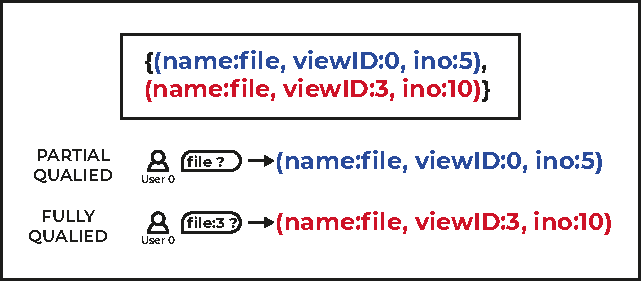
\includegraphics[scale=0.6]{Le-bonhomme-sait-pas-ce-quil-veut.pdf}
\end{figure}


\subsection{Divergent renames}

Without coordination, \textit{mkdir} and \textit{mknod} are not the only
operations that can create a link. (See section~\ref{fs:weak} for problematic
renames).

Because of this situation, using a counter to track the number of links is no
longer sufficient because at the time we issue the \texit{rename} operation
we cannot know if the operation will end up being concurrent.

To keep track of the number of links, we use another RWSet that is
always updated alongside the directory entries updates.

Each link contains the parent inode number and the FQN which contains
the ViewID.
We use the ViewID again to have the exact same semantics as the set storing
the directory entries. Thus the link set is always valid with respect to
links currently visible in the FS.

However, this solution by itself is not sufficient to ensure that directories have a
unique parent at all times.

This is solved with an additional Last Writer Win register that serves us as
an arbitrator to decide which link is valid.

Each time we load directories  entries, we check the parent register of each
entry that points to a directory. If the entry comes from a parent that doesn’t
match the value of the register, it is garbage collected and never shown to the user.
Because the register is always updated inside the same transaction, the
value of the register always matches the update that add the entry
to the parent.

\subsection{A simple conflict scenario}

Using the design described above we can imagine how ElmerFS behaves in case
of a conflict.

To illustrate this, let's consider again Bob and Alice. Alice and Bob work
on the same project but cannot communicate. They do not want to wait and start by creating a
folder named \textit{projectA}. Because the project will likely needs a report,
they both create a report file \textit{report.doc} to enter their early work.

Once the connection reestablished, Bob see that there is now two folders:
his own folder \textit{projectA} and another one \textit{projectA:Alice}.

They can both continue to work on their project without worrying about
conflict or implicit merges. After some time Bob and Alice agree to merge
their work. Alice remove its old no longer relevant folder.

They both see a unique file tree \textit{projectA/report.doc}.

This sequence is very close to what a user might expect when working with
a local file system.

\begin{figure}[h]
	\caption{Alice and Bob conflict scenario.}
	\Description{Alice and Bob creates a folder without a connection,
				 they both see their own folder with the original name
				 and the one in conflict}
	\centering
	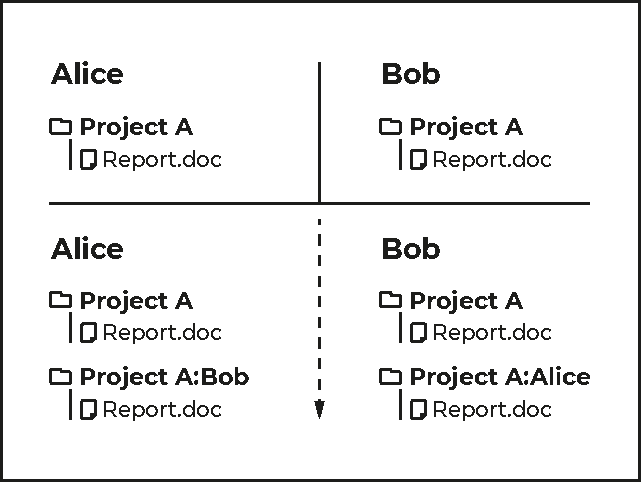
\includegraphics[scale=0.5]{AliceBob-font-des-fichiers.pdf}
\end{figure}

\section{Direction for future research}
\label{crdt:future}

\subsection{Concurrent ino number generation and recycling}

Our solution to generate an inode number described in section~\ref{sec:generation_inode_number}
is not truly concurrent.
To address this, and to be able to recycle inode numbers,
a specialized CRDT type might be needed.
A possible solution for specifying such a CRDT type would be to draw inspiration
from sequence CRDT used for text processing application where each inserted
character is assigned an unique position \cite{nedelec2013lseq, letia2009crdts}.

\subsection{Cycle with concurrent rename}

Our implicit hierarchy using map CRDTs does not prevent the creation of cycles.
Some CRDT tree design exists~\cite{martin2012abstract} but relies on multiple correction
layers that perform additional operations to recover from the broken invariants.
We believe that both this issue could be solved by the use of a conditional transaction framework.
The key idea would be to merge operations only if they satisfy a specified condition.

For cycles, this would simply be that the resulting tree does not have a cycle.
Transactions that do not satisfy this condition should be discarded
in a deterministic manner to ensure convergence.

\subsection{Dealing with Orphan CRDTs}

Our deletion strategy relies solely on issuing a delete operation for all
known CRDTs of an entity.

For file content, where we store an implicit and unbounded number of CRDT,
concurrent add operations merges can lead to content lingering
without an entity to reference it.

Tombstones are sometimes used in CRDT design, but here we need a mechanism
to link and propagate deletion across multiple CRDT.

We are not aware of any protocol that allows this.
A possible framework could rely on a unique tombstone and use conditional
transactions described in the previous section to discard concurrent
add operations.

\section{Conclusion}

In the paper, we explore the challenges in the design of a truly
concurrent shared geo-replicated file systems under weak consistency,
and present the design of ElmerFS, a CRDT-based file system.

Conflict resolution in ElrmerFS is based on the goal of preserving user
intention.
ElmerFS ensures all file system replicas eventually converge to the same state,
while also allowing users to complement or reverse the results of conflict resolution
through a simple interface that preserves the standard file system POSIX semantics.

We have implemented a prototype of ElmerFS and are in the process of performing
experimental evaluation.

While there remain open problems to be addressed,
we believe that leveraging the properties of CRDTs is a promising path towards
highly available and truly concurrent file systems and believe that future
work should go in this direction.

\bibliographystyle{ACM-Reference-Format}
\bibliography{elmerpap}

\end{document}
